\documentclass[11pt,titlepage]{article}
\usepackage{mathtools}
\usepackage{amsmath}
\usepackage{amssymb}
\usepackage{amsthm}
\usepackage{mathtools}
\usepackage{blindtext}
\usepackage{enumitem}
\usepackage[linesnumbered,ruled,vlined]{algorithm2e} 
\usepackage[margin=2.56cm]{geometry}
\usepackage{csc}
\usepackage{changepage}
\usepackage{mathtools}
\usepackage{listings}
\usepackage{xcolor}
\usepackage{todonotes}
\usepackage{graphicx}
\usepackage{subcaption}
\usepackage{float}
\usepackage{hyperref}
\usepackage{url}
\usepackage[style=ACM-Reference-Format,backend=bibtex,sorting=none]{biblatex}
\addbibresource{references.bib}



\title{CSC420 Project Report \\ Super Resolution}
\author{Team: Tree Wizards}
\date{Adam Adli, Linwen Huang, Jason Tang}

\setlength\parindent{0pt}
\begin{document}
\maketitle
% RUBRIC
% Abstract (1)
% Introduction and Literature Review
%     Introduction to the problem (1.5)
%     Range, depth, and quality of literature research on your topic (2)
% Methodology, Results, and Experiments
%     Theoretical part (1.5)
%     Empirical work (Quality of Analyses) (2.5)
%     Presentation of Results/Failures (2.5)
% Conclusion (2)
% Author's Contributions (0.5)
% References (0.5)
% The overall quality of the report(1)

\section*{Abstract}

Super-resolution is an extremely difficult computer vision problem that has seen considerable breakthroughs in recent literature; some interesting solution have been developed through the use of deep learning on generative adversarial networks (GAN) to upsample images with high perceptual quality. SRResNet and SRGAN are two examples of state-of-the-art neural networks that produce high-fidelity image upsampling. Recent breakthroughs have been made in hyper-parameter optimization with literature discussing a new optimization method called Delta-STN. In this paper, we present our attempt at applying Delta-STN optimization to SRResNet while exploring the efficiency of transfer-learning on a dataset we prepared. Through this approach, we document considerations we made regarding dataset preparation, Delta-STN application, and neural network implementation.

\section*{Introduction and Literature Review}
\subsection*{The Problem}
The problem of super resolution (SR) aims to generate a high-resolution (HR) version image from one or more low resolution (LR) versions of the image. Using a single LR image is referred to as single image super resolution (SISR), and similarly, using multiple LR images is referred to as multi-image super resolution (MISR) \cite{Yang2019}.

\bigskip

Often the ability to generate an HR image is useful as it can provide more valuable details, which is important in a variety of fields such as medical imaging, satellite imaging, and image/video enhancement [1, 2]. This can also lead to reduced bandwidth required to transmit images and video, which make up a significant amount of the information transmitted throughout the internet. Traditional methods for upscaling have usually relied on methods such as interpolation. While these methods are simple to implement, they often produce subpar results. 

\begin{figure}[hp]
  \centering
  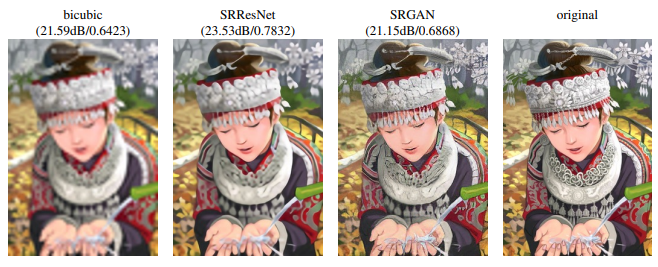
\includegraphics[width=\linewidth]{sr_examples.png}
  \caption{Examples of images processed by 3 different SR models: bicubic, SRResNet, SRGAN \cite{Ledig2017}}
  \label{fig:sr_eg}
\end{figure}

\subsection*{Relevant Research}

There have been many approaches to the SR problem. Traditionally there are three main types of SISR algorithms: interpolation based, reconstruction-based and learning-based \cite{Yang2019}.Examples of interpolation-based algorithms include the bicubic interpolation and Lanczos resampling. Reconstruction based methods such as those by Dai et al., Sun et al., Yan et. Al. And Marquina et. Al have been used by restricting the solution space to generate HR images \cite{Yang2019}. Learning-based methods have been used by Freeman et al. and Chang et al. These methods employ machine learning algorithms to analyze the statistical relationships between an LR image and a HR image using training examples \cite{Yang2019}. However, these approaches have suffered from shortcomings, such as accuracy and generalizability issues in addition to lack of scalability. In recent years, the focus in SISR has been with deep learning-based methods which have shown significant improvements in results compared to older methods \cite{Yang2019}.

\bigskip

In the last few years, the application of deep learning convolutional neural networks (CNNs) has become prominent \cite{Yang2019}. This has lead to the creation of SR models known as SRCNNs. The focus of our project however looks at another type of deep learning SR model, the SRGAN, created by Ledig et al. \cite{Ledig2017} SRGANs are super resolution models that use generative adversarial networks (GANs) are a type pf generative model that uses supervised learning. There are two networks associated SRGANs, the generator network and the discriminator network. During training a HR image is down sampled to a LR image. The image is then passed to the generator network which attempts to upsample the imae to create a SR image. The discriminator then attempts to distinguish between the SR image and the ground truth HR image. The discriminator then backpropagates the GAN loss to train the discriminator and the generator (to create SR images more reflective of the ground truth images) \cite{Hui2018}. Another network is the SRResNet which is the same model as SRGAN but just without the GAN portion \cite{Hui2018}. 

\begin{figure}[hp]
  \centering
  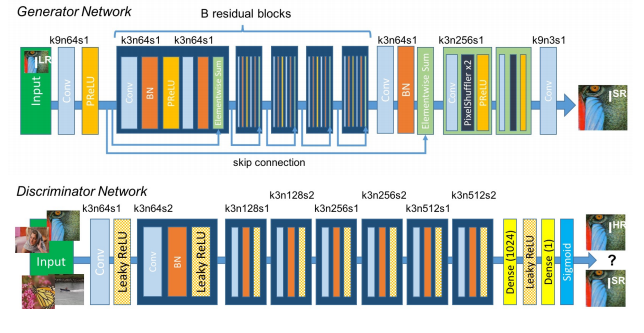
\includegraphics[width=\linewidth]{srgan_arch.png}
  \caption{SRGAN architecture used by Ledig et al. \cite{Ledig2017}}
  \label{fig:srgan}
\end{figure}

\bigskip
The generator network uses residual blocks originated by ResNet, within  each residual block is two convolutional layers \cite{Hui2018}. ResNet introduces skip connections aka shortcut connections which allows for deeper networks. This helps to alleviate the issues that arise when deep CNNs have too many layers \cite{Tsang2018}. The residual block uses small 3x3 kernels and 64 feature maps, followed by batch-normalization and Parametric ReLU \cite{Hui2018}. In the discriminator network a Leaky Relu is used. The network contains 8 convolutional layers, and mimics the structure seen in the VGG network \cite{Hui2018}. This results in 512 feature maps followed by 2 dense layers and a sigmoid activation function \cite{Hui2018}. SRGAN also uses a perceptual loss function, which is the waited sum of the content loss and an adversarial loss component \cite{Hui2018}.

\begin{figure}[hp]
  \centering
  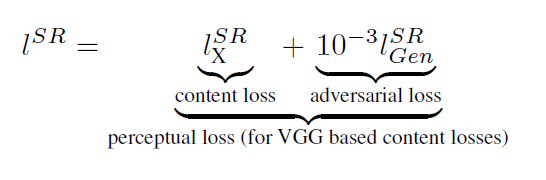
\includegraphics[width=0.8\linewidth]{perceptual_loss.png}
  \caption{Perceptual loss function used in SRGAN \cite{Hui2018}.}
  \label{fig:srgan}
\end{figure}

Instead of using MSE loss for content loss SRGAN uses VGG loss, which is the euclidean distance between the feature representation of the SR generated image and the ground truth HR image \cite{Hui2018}. The content loss uses perceptual similarity instead of pixel space similarity \cite{Hui2018}. The adversarial loss is based on the probablities (the probablity the SR generated image is a ground truth HR image) of the discriminator over all training samples. As such the adversarial loss pushes our SR generated image closer to the ground truth HR image \cite{Hui2018}.


\bigskip

SRGAN outperforms traditional and CNN based SR models. It was also one of the first models that could infer photo realistic images with a 4x upscaling factor. As a result SRGAN shows state of the art results, and produces extremely high detailed textured images. SRGAN also scored extremely well in mean opinion score tests compared to other models \cite{Tsang2020}. SRResNet also outperformed models in PSNR and SSIM \cite{Tsang2020}.

\bigskip

While SRGAN and SRGAN-based neural networks provide state-of-the-art SISR, it is still not a perfect solution. It can still be susceptible generalizability issues depending on training data set \cite{Tsang2020}. Additionally, SRGAN may be highly effective at high-frequency texture generation while introducing artifacts that may distort text \cite{Kanska2017}. Furthermore, the use of residual blocks come with a computational cost in exchange for higher accuracy in SRGAN models like SRResNet \cite{Kanska2017}. Making them even more difficult to develop in face of computational cost, GAN-based networks are known to be difficult to transfer-learn \cite{frégier2020mind2mind}. With these trade-offs in mind there is still heavy research underway in the domain of SISR and its use of general adversarial networks.

\bigskip

Delta-STN by Juhan Bae and Roger Grosse presents a novel approach for automating the tuning of regularization hyperparameters such as dropout, weight decay, and data augmentation values \cite{Bae2020}. It improves upon conventional methods such as random search, grid search, and Bayesian Optimization by utilizing a hypernetwork to approximate the best response function. This can be especially useful in SISR since learning optimal hyperparameter values for data augmentation could better regularize the model and allow it to better generalize to unseen data.

\section*{Methodology, Results, and Experiments}
\subsubsection*{Sources}
The pretrained weights and a portion of our codebase is based on \href{https://github.com/dongheehand/SRGAN-PyTorch}{Donghee Son's unofficial implementation} on Github \cite{SonGitHub}. Our main extensions are our methods for dataset processing and transfer learning the pretrained weights. 

\subsubsection*{Dataset Preperation}
A standard dataset used for super-resolution training and evaluation is the DIV2K dataset, which is the one our pretrained weights were trained upon. There are some considerations that must be made when preparing a super-resolution dataset. Namely, we want to ensure that the dataset is complex enough in detail to show the power of Super Resolution, but we also require that the dataset is small enough in size to train in a reasonable amount of time. We also found that using photos with JPEG compression would yield artifacts when input into super-resolution models as they are less trivial to use due to blocking artifacts; so we also limited our choices to uncompressed file formats \cite{10.1007/978-3-319-95957-3_50}.\\

To accomplish this, we chose a dataset of ~800 Pokemon. Within it, there are some images that are image and with a low level of detail, and there are some of which are fairly complex and detailed. We then resized the original $475 \times 475$ images into $256 \times 256$ high resolution images, which we then scaled down by a factor of 4 to get $64 \times 64$ low resolution images. Both these operations were performed using Bicubic interpolation with the Pillow library. The smaller sizes allowed us to train both faster and with more stability due to the ability to use larger batch sizes.\\

The final action we performed on the data prior to actual training was data augmentation. Specifically, we used randomized affine and homography transformations to alter the perspective and view of the original image, as we learned in lecture. Performing this allowed us to essentially create new altered images for each training iteration, thereby reducing the possibility of our model overfitting to the small number training samples. Otherwise, it would be possible for our model, with its large parameter capacity, to memorize data points rather than actually learn how to perform super resolution, leading to degraded generalization performance on non-training data.


\subsection*{Experiments}
Focusing on SRGAN and SRResNet neural network architectures, we took an exploratory approach to our project attempting to expand on existing work through different objectives:
\begin{enumerate}
    \item prepare a dataset for super-resolution learning.
    \item conduct transfer-learning using our prepared dataset using SRResNet.
    \item experiment with Delta-STN.
\end{enumerate}
Although we made considerable progress on our objectives, we ran into some challenges that hindered our final results. Nonetheless, we gained some insights that we document.\\

First, as described in the previous section, we were able to successfully prepare our dataset of Pokemon for use in transfer learning with the pretrained weights. We were then able to create a training loop in which we fine tuned these pretrained weights, resulting in a noticeable increase in performance, as we show in the following section. Lastly, we ran into time and compute challenges with incorporating the Delta-STN implementation into our SISR model so we leave it as an avenue for further research and exploration.

\subsection*{Results}
Below are several selected example predictions and metric evaluations of images in the test set. The values in the brackets represent PSNR (Peak signal-to-noise ratio) and Perceptual Loss (MSE on the outputs of VGG19 layer 5-4).
\begin{figure}[H]
    \centering
    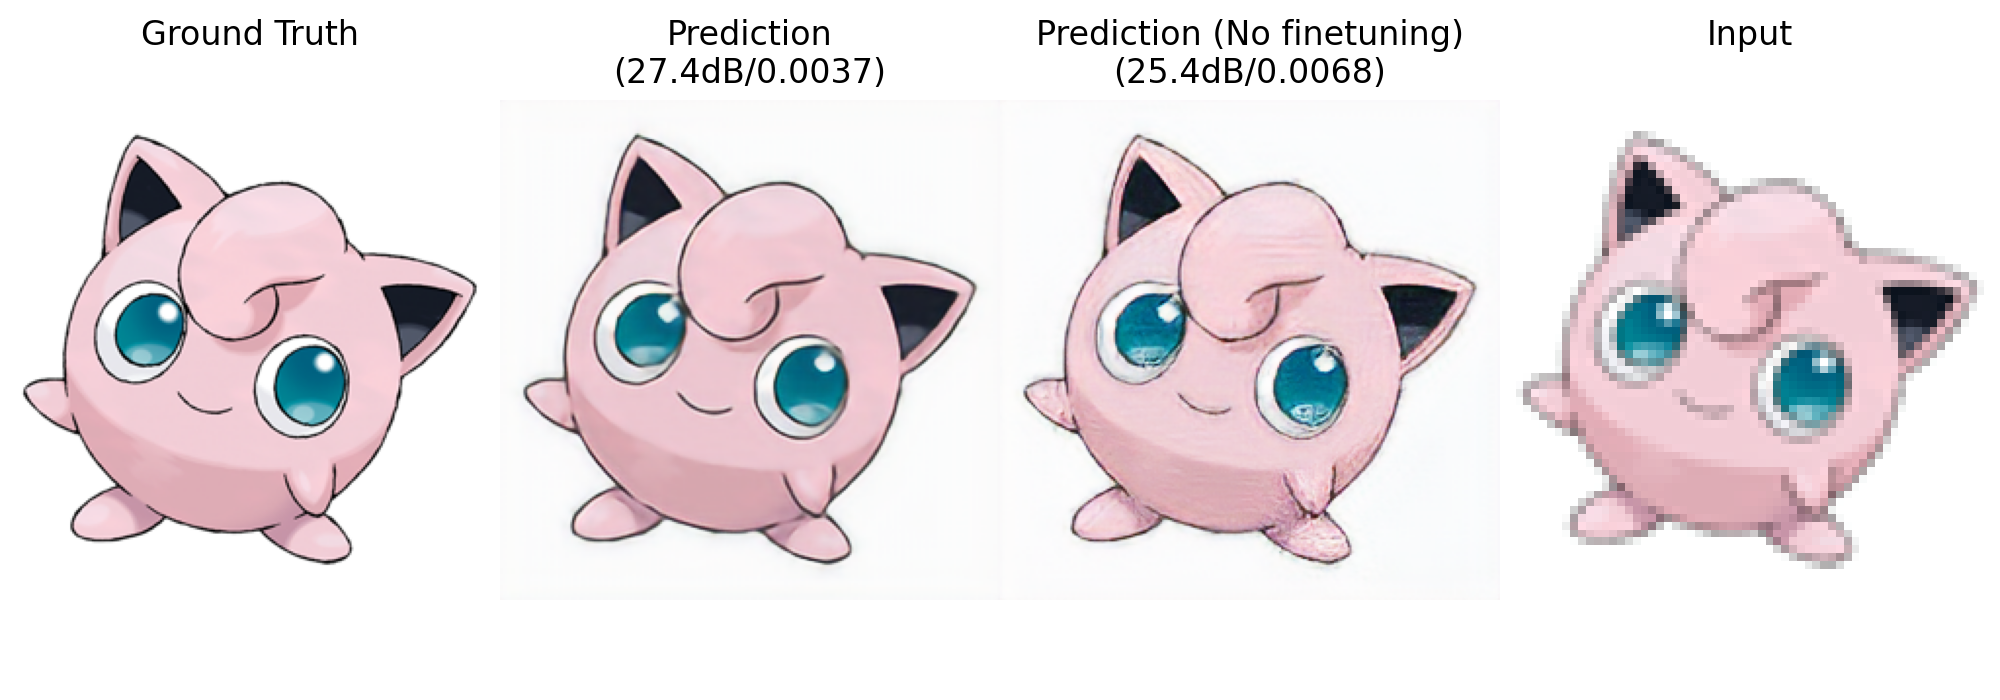
\includegraphics[width=0.93\textwidth]{results/039.png}
\end{figure}
\begin{figure}[H]
    \centering
    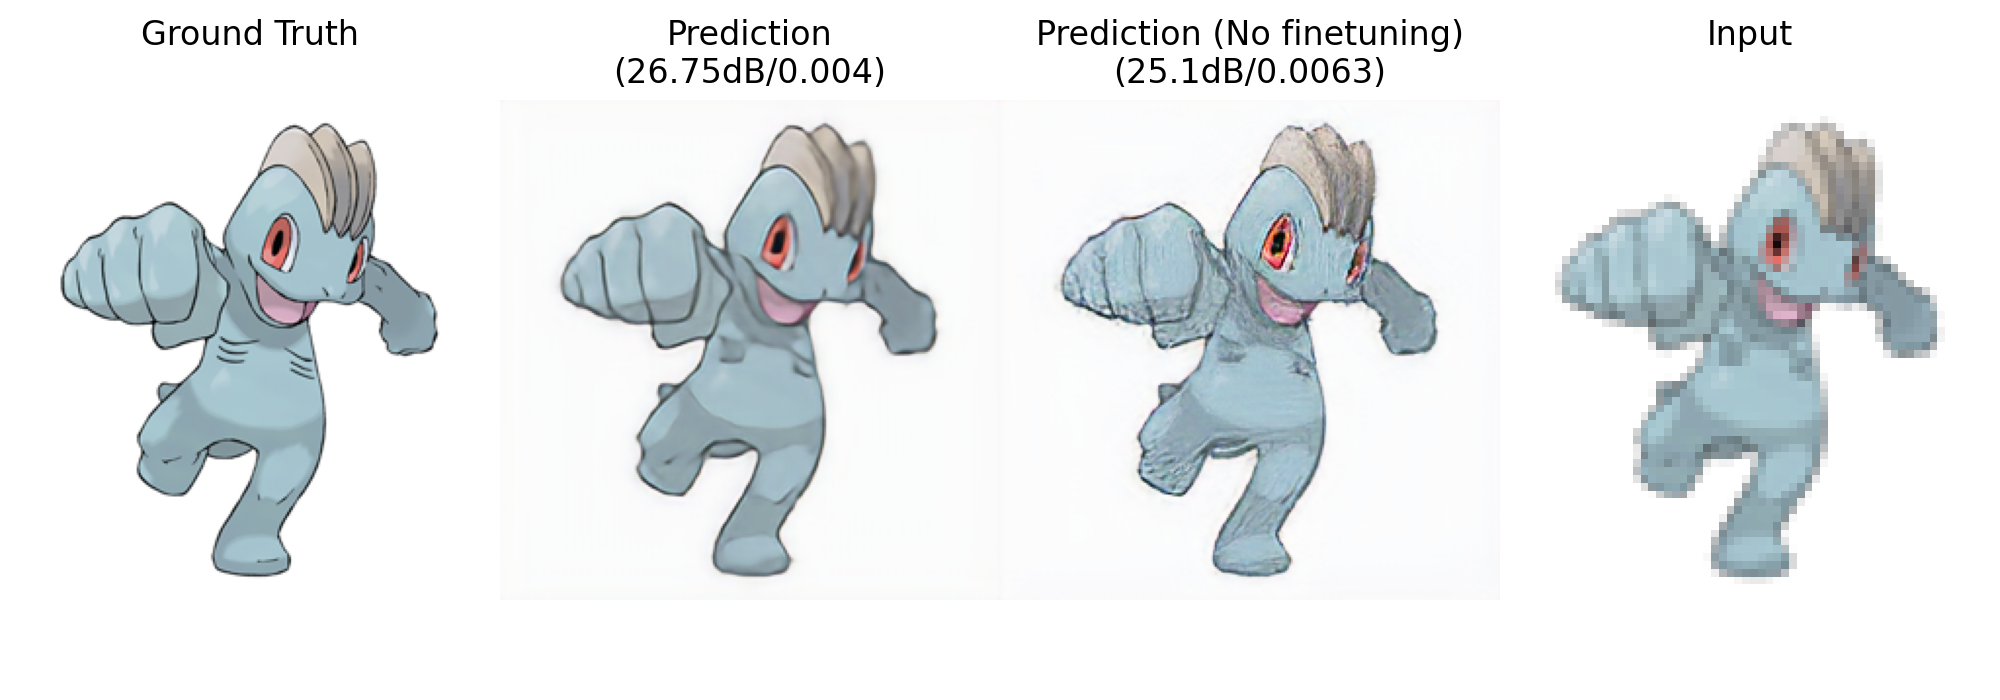
\includegraphics[width=0.93\textwidth]{results/066.png}
\end{figure}
\begin{figure}[H]
    \centering
    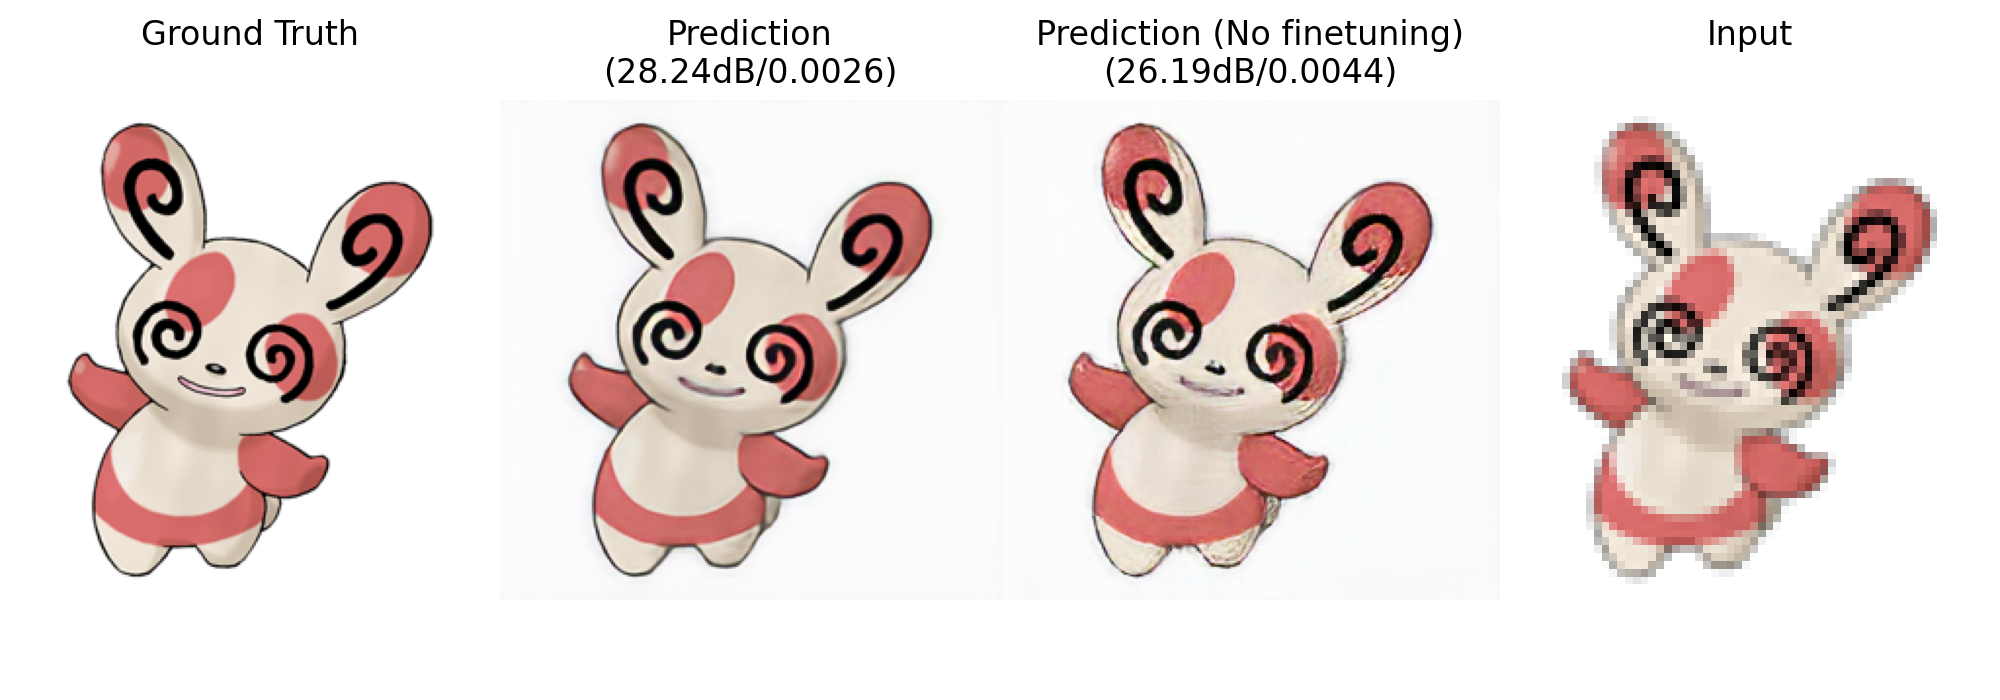
\includegraphics[width=0.93\textwidth]{results/327.png}
\end{figure}
\begin{figure}[H]
    \centering
    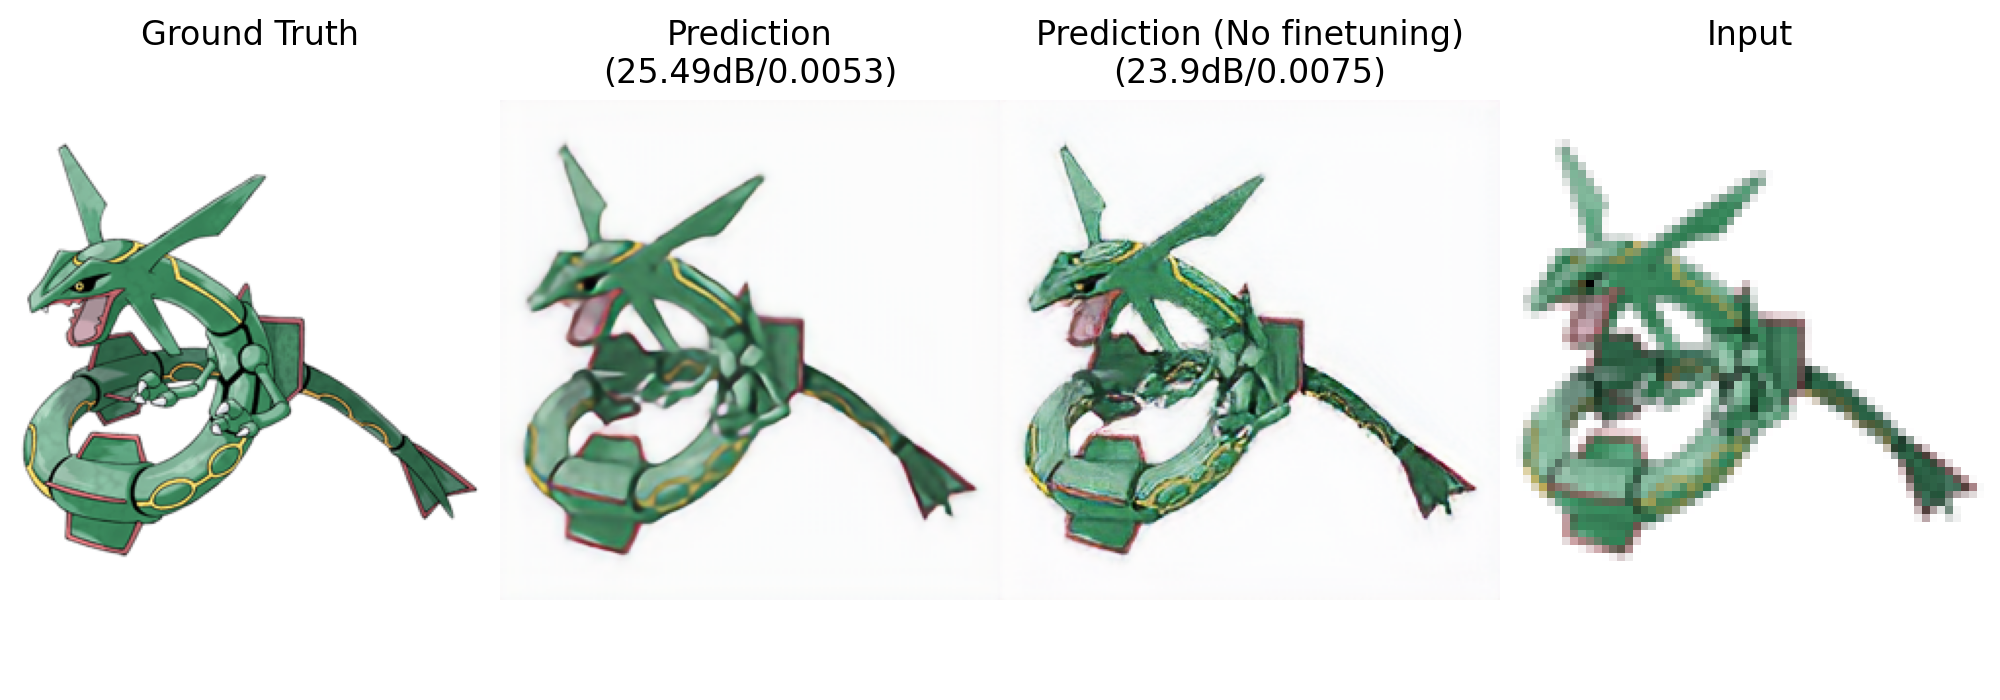
\includegraphics[width=\textwidth]{results/384.png}
\end{figure}
\begin{figure}[H]
    \centering
    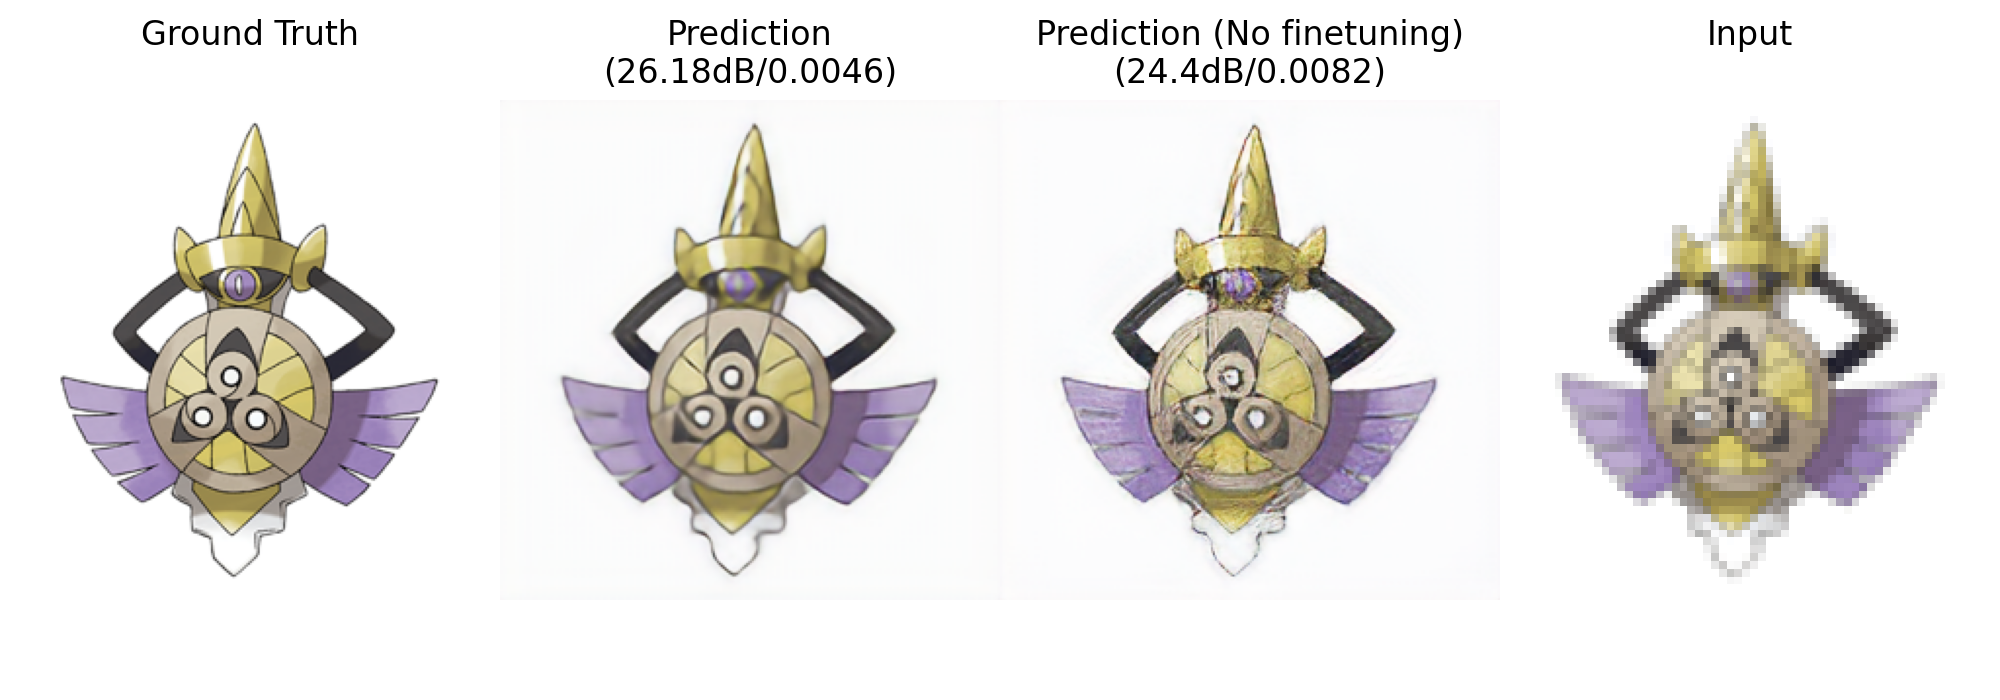
\includegraphics[width=\textwidth]{results/681_f2.png}
\end{figure}
\begin{figure}[H]
    \centering
    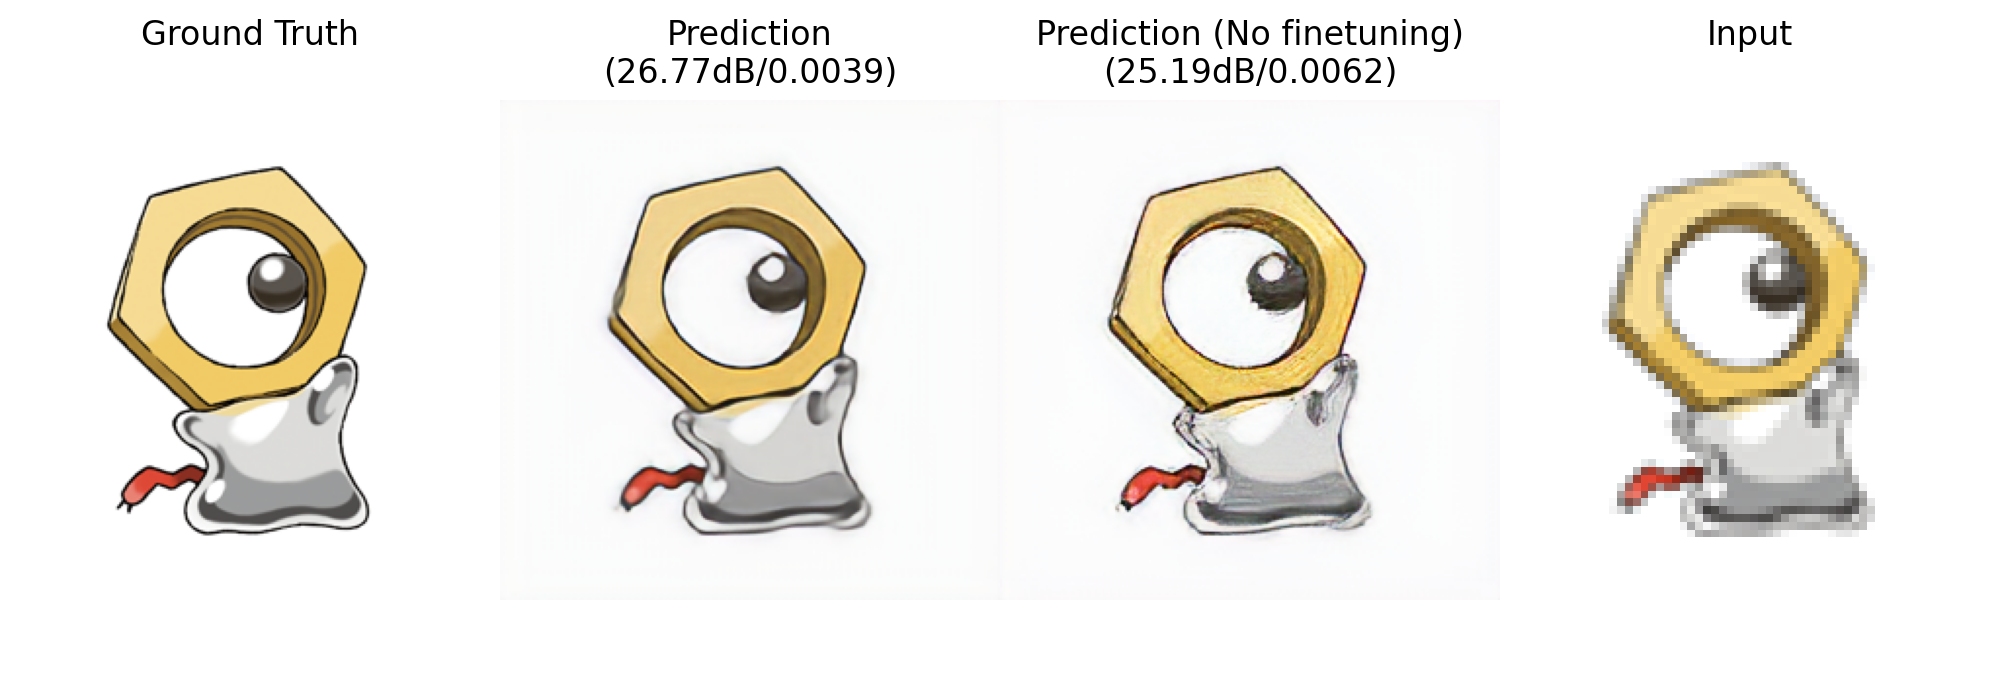
\includegraphics[width=\textwidth]{results/808.png}
\end{figure}

Below are the averaged performance on various metrics for images in the validation set. 
\begin{center}
\begin{tabular}{|c|c|c|c|c|}
     \hline
     & MSE & PSNR & VGG22 & VGG54\\
     \hline
     Without finetuning & 0.002561 & 27.2486 & 0.015313 & 0.004093\\
     With finetuning & 0.002394 & 27.4498 & 0.012861 & 0.003504\\
     \hline
\end{tabular}
\end{center}

\section*{Conclusion}

Overall, we were able to slightly improve the scores achieved using MSE and PSNR, as well as improving both perceptual losses and MSE loss between output features at certain layers of the VGG19 model. In our results we also saw that our model was able to remove artifacts that were found in the non-finetuned model without sacrificing too much image sharpness. This increase in performance can be attributed to the various forms of regularization we introduced during the training of our model. For example, the affine transformations applied to augment our data, and the application of fine tuning models in parallel with an adversarial network.\\

Though we met many difficulties and obstacles in this project, we have learned a lot as a result. Specifically, we became more familiar with the different models and techniques in the field of downsampling and Super Resolution, as well as the various types of dataset preparation and data considerations to be made. Additionally, we became better acquainted with the PyTorch ML library, other implementation tools/frameworks, and the basic principles behind implementing and training neural networks.

%In the previous section, we note that we were able to slightly improve on all metrics, with better MSE and PSNR performances as well as on both perceptual losses, an MSE loss between output features at certain layers of the VGG19 model. We also note the qualitative improvement of the results in the removal of the frequent artifacts found in the non-finetuned model outputs while not sacrificing too much sharpness in order to achieve this. We can attribute this increase in performance with unseen data (all images shown are from the test set) to the various forms of regularization we introduced throughout the training of the models, ranging from affine transforming the data during data augmentation to finetuning models in parallel with an adversarial network.

\section*{Author Contributions}

\subsection*{Adam Adli}
\begin{itemize}
    \item Research of models/pretrained weights
    \item Sourced pokemon datasource
    \item Set up code base for SRGAN/SRResNet
    \item Wrote Python scripts involved with using pretrained weights, data processing and modified source code for SRGAN/SRResNet
    \item Wrote up proposal and report
\end{itemize}

\subsection*{Linwen Huang}
\begin{itemize}
    \item Research of models/pretrained weights
    \item Sourced pokemon datasource
    \item Wrote python scripts used in generating LR images/data processing and modified source code for SRGAN/SRResNet
    \item Created presentation slide deck, wrote up proposal and report
\end{itemize}

\subsection*{Jason Tang}
\begin{itemize}
    \item Performed transfer learning on the pretrained weights
    \item Set up data augmentation pipeline
    \item Wrote class to evaluate multiple metrics on various datasets
    \item Attempted initial experiments with Delta-STN
    \item Wrote up proposal and report
\end{itemize}

% \section*{References}
% \sloppy 
% \begin{enumerate}
% \item W. Yang, X. Zhang, Y. Tian, W. Wang, and J.-H. Xue, “Deep Learning for Single Image Super-Resolution: A Brief
% Review,” arXiv.org, 12-Jul-2019. [Online]. Available: https://arxiv.org/abs/1808.03344. [Accessed: 04-Nov-2020].

% \item K. Kańska, “Using deep learning for Single Image Super Resolution,” deepsense.ai, 25-Apr-2019. [Online]. Available: https://deepsense.ai/using-deep-learning-for-single-image-super-resolution/. [Accessed: 04-Nov-2020].

% \item S.-J. Park, H. Son, S. Cho, K.-S. Hong, and S. Lee, “SRFeat: Single Image Super-Resolution with Feature Discrimination,” Computer Vision – ECCV 2018 Lecture Notes in Computer Science, pp. 455–471, 2018. [Online]. Available:
% https://link.springer.com/chapter/10.1007/978-3-030-01270-0\_27. [Accessed: 04-Nov-2020].

% \item B. Lim, S. Son, H. Kim, S. Nah, and K. M. Lee, “Enhanced Deep Residual Networks for Single Image Super-Resolution,” 2017 IEEE Conference on Computer Vision and Pattern Recognition Workshops (CVPRW), Jul. 2017. [Online]. Available: https://arxiv.org/abs/1707.02921. [Accessed: 04-Nov-2020].

% \item C. Ledig, L. Theis, F. Huszar, J. Caballero, A. Cunningham, A. Acosta, A. Aitken, A. Tejani, J. Totz, Z. Wang, and W. Shi, “Photo-Realistic Single Image Super-Resolution Using a Generative Adversarial Network,” 2017 IEEE Conference on Computer Vision and Pattern Recognition (CVPR), 2017. [Online]. Available: https://arxiv.org/abs/1609.04802. [Accessed: 04-Nov-2020].

% \item Hui, Jonathan. "GAN-Super Resolution GAN (SRGAN)". Jun 15 2018. Available:  https://jonathan-hui.medium.com/gan-super-resolution-gan-srgan-b471da7270ec [Accessed: 18-12-2020]

% \item Tsang, Sik-Ho. "Review: ResNet - Winner of ILSVRC 2015 (Image Classification, Localization, Detection)". Sep 15 2018. Available: https://towardsdatascience.com/review-resnet-winner-of-ilsvrc-2015-image-classification-localization-detection-e39402bfa5d8 [Accessed: 18-Sep-2020].

% \item Tsang, Sik-Ho. "Review: SRGAN * SRResNet - Photo-Realistic Super Resolution (GAN & Super Resolution)". Apr 22 2020. Available:https://sh-tsang.medium.com/review-srgan-srresnet-photo-realistic-super-resolution-gan-super-resolution-96a6fa19490 [Accessed: 18-Dec-2020].

% \item N. Takano and G. Alaghband, “SRGAN: Training Dataset Matters,” Computing Research Repository (CoRR), Mar. 2019.
% [Online]. Available: https://arxiv.org/abs/1903.09922. [Accessed: 04-Nov-2020].

% \item Grosse, Roger and Bae Juhan. "Delta-STN: Efficient Bilevel Optimization for Neural Networks using Structured Response Jacobians." Neurips 2020, Oct 26 2020. [Online]. Available: https://arxiv.org/abs/2010.13514 . [Accessed: 08-Dec-2020].
% \end{enumerate}

% [1]: \cite{Yang2019}\\
% [2]: \cite{Kanska2017}\\
% [3]: \cite{Park2018}\todo{NOT USED: S.J. Park, LIM [3] and [4] [9]}\\
% [4]: \cite{Lim2017}
% [5]: \cite{Ledig2017}
% [6]: \cite{Hui2018}
% [7]: \cite{Tsang2018}
% [8]: \cite{Tsang2020}
% [9]: \cite{Takano2019}
% [10]: \cite{Bae2020}
% \newpage
% \bibliographystyle{acm}
% \bibliographystyle{plainurl}
% \bibliography{references.bib}

\newpage
\printbibliography



\end{document}